\chapter{Boilerplate for Graph}\label{chap:graph_boilerplate}
\section{Graph (Universal)}
This section explores the {\color{blue}{universal implementation}} of a graph, where the {\color{blue}{graph}}, its {\color{blue}{nodes}}, and {\color{blue}{edges}} are all implemented as classes.

\subsection{Directed Graph}
\subsubsection{Data Structures Interfaces}
\begin{lstlisting}
class Node {
 public:
	Node(int val) : val(val) {}
	
	int val;
	std::vector<Edge*> in_edges_;
	std::vector<Edge*> out_edges_;
};

class Edge {
 public:
	Edge(Node* src, Node* dst) : src_(src), dst_(dst) {}
	
	Node* src_;
	Node* dst_;
};

class Graph {
 public:
  Graph() = default;

  void DFSRecursive(std::vector<Node*>& start_nodes);
  void DFSVisit(Node* node, std::unordered_set<Node*>& visited);
  void DFSIterative(std::vector<Node*>& start_nodes);
  void BFS(std::vector<Node*>& start_nodes);

  bool IsCyclicWithoutPruining();
  bool DetectCycleFromNodeWithoutPruining(Node* node, std::unordered_set<Node*>& path);
  bool IsCyclic();
  bool DetectCycleFromNode(Node* node, std::unordered_set<Node*>& path,
                           std::unordered_set<Node*>& visited);

  std::vector<Node*> SourceNodes();
  std::vector<Node*> SinkNodes();

  void Connect(Node* src, Node* dst);

  std::vector<Node*> nodes_;
  std::vector<Edge*> edges_;
};
\end{lstlisting}

\subsubsection{DFS - Recursive}
\begin{lstlisting}
void Graph::DFSRecursive(std::vector<Node*>& start_nodes) {
  // we can guarantee visited vector is always up to date because it is passed by reference
  std::unordered_set<Node*> visited;
  for (auto node : start_nodes) {
    if (visited.find(node) == visited.end()) { DFSVisit(node, visited); }
  }
}

void Graph::DFSVisit(Node* node, std::unordered_set<Node*>& visited) {
  if (!node) { return; }
  // handle the node, e.g., print it
  std::cout << node->val << " ";
  visited.insert(node);
  // for each neighbor
  for (auto edge : node->out_edges_) {
    Node* dst = edge->dst_;
    if (visited.find(dst) == visited.end()) { DFSVisit(dst, visited); }
  }
}
\end{lstlisting}

\subsubsection{DFS - Iterative}
\begin{lstlisting}
void Graph::DFSIterative(std::vector<Node*>& start_nodes) {
  std::stack<Node*> stk;
  std::unordered_set<Node*> visited;
  for (auto node : start_nodes) {
    stk.push(node);
    visited.insert(node);
  }
  while (!stk.empty()) {
    Node* top = stk.top();
    stk.pop();
    // handle the node, e.g., print it
    std::cout << top->val << " ";
    // for each neighbor
    for (auto edge : top->out_edges_) {
      if (visited.find(edge->dst_) == visited.end()) {
        stk.push(edge->dst_);
        visited.insert(edge->dst_);
      }
    }
  }
}
\end{lstlisting}
\subsubsection{BFS}\label{subsubsec:graph_universal_implementation_bfs}
\begin{tcolorbox}[title=\textbf{Takeaway}, width=1.0\linewidth,]
When designing a BFS algorithm, you should:
\begin{itemize}
\item Carefully check the neighboring nodes, {\color{blue}{only enqueue valid nodes}} for exploration.
\item For any states influencing the decision to explore the neighboring nodes, update them as soon as possible, ideally {\color{blue}{at the moment of its enqueuing}}. This can avoid enqueuing duplicate nodes and thus prevent unnecessary explorations.
\end{itemize}
\end{tcolorbox}

The only difference between Version 1 and Version 2 lies in the timing of marking the visited nodes.
\begin{itemize}
\item Version 1 marks nodes as visited {\color{blue}{immediately after enqueuing them}}.
\item Version 2 marks nodes as visited {\color{blue}{only after dequeuing them}}.
\end{itemize}
This state influences whether or not BFS decides to explore its neighbors. A smart choice is to mark visited nodes as early as possible. If we wait too long to mark them, we might end up with enqueuing duplicate nodes again and again, which reduces the algorithm's speed.\\

Version 1 (You should always choose this version.)
\begin{lstlisting}
void Graph::BFS(std::vector<Node*>& start_nodes) {
  std::queue<Node*> q;
  std::unordered_set<Node*> visited;
  for (auto node : start_nodes) {
    q.push(node);
    visited.insert(node);
  }
  while (!q.empty()) {
    Node* front = q.front();
    q.pop();
    // handle the node, e.g., print it
    std::cout << front->val << " ";
    // for each neighbor
    for (auto edge : front->out_edges_) {
      if (visited.find(edge->dst_) == visited.end()) {
        q.push(edge->dst_);
        visited.insert(edge->dst_);
      }
    }
  }
}
\end{lstlisting}

Version 2 (Don't use this version.)
\begin{lstlisting}
void Graph::BFS(std::vector<Node*>& start_nodes) {
  std::queue<Node*> q;
  std::unordered_set<Node*> visited;
  for (auto node : start_nodes) {
    q.push(node);
    visited.insert(node);
  }
  while (!q.empty()) {
    Node* front = q.front();
    q.pop();
    if (visited.find(front) != visited.end()) { continue; }
    // handle the node, e.g., print it
    std::cout << front->val << " ";
    visited.insert(front);
    // for each neighbor
    for (auto edge : front->out_edges_) {
      if (visited.find(edge->dst_) == visited.end()) { q.push(edge->dst_); }
    }
  }
}
\end{lstlisting}

\subsubsection{Detect Cycles}
Brute-Force Backtracking (Don't use this version)
\begin{lstlisting}
bool Graph::IsCyclicWithoutPruining() {
  std::unordered_set<Node*> path;
  for (auto node : nodes_) {
    if (DetectCycleFromNodeWithoutPruining(node, path)) { return true; }
  }
  return false;
}

bool Graph::DetectCycleFromNodeWithoutPruining(Node* node, std::unordered_set<Node*>& path) {
  // base case - null node
  if (!node) { return false; }
  // base case - cycle detected
  if (path.find(node) != path.end()) { return true; }
  path.insert(node);
  for (auto edge : node->out_edges_) {
    if (DetectCycleFromNodeWithoutPruining(edge->dst_, path)) { return true; }
  }
  path.erase(node);
  return false;
}
\end{lstlisting}

Add pruning (You should always choose this version)
\begin{lstlisting}
bool Graph::IsCyclic() {
  std::unordered_set<Node*> path;
  // nodes that have been explored and not in any cycle
  std::unordered_set<Node*> visited;
  for (auto node : nodes_) {
    if (DetectCycleFromNode(node, path, visited)) { return true; }
  }
  return false;
}

bool Graph::DetectCycleFromNode(Node* node, std::unordered_set<Node*>& path,
                                std::unordered_set<Node*>& visited) {
  // base case - null node
  if (!node) { return false; }
  // base case - cycle detected
  if (path.find(node) != path.end()) { return true; }
  // pruning - visited node
  if (visited.find(node) != visited.end()) { return false; }
  path.insert(node);
  visited.insert(node);
  for (auto edge : node->out_edges_) {
    if (DetectCycleFromNode(edge->dst_, path, visited)) { return true; }
  }
  path.erase(node);
  return false;
}
\end{lstlisting}

\subsubsection{Example}
\begin{figure}[H]
\centering
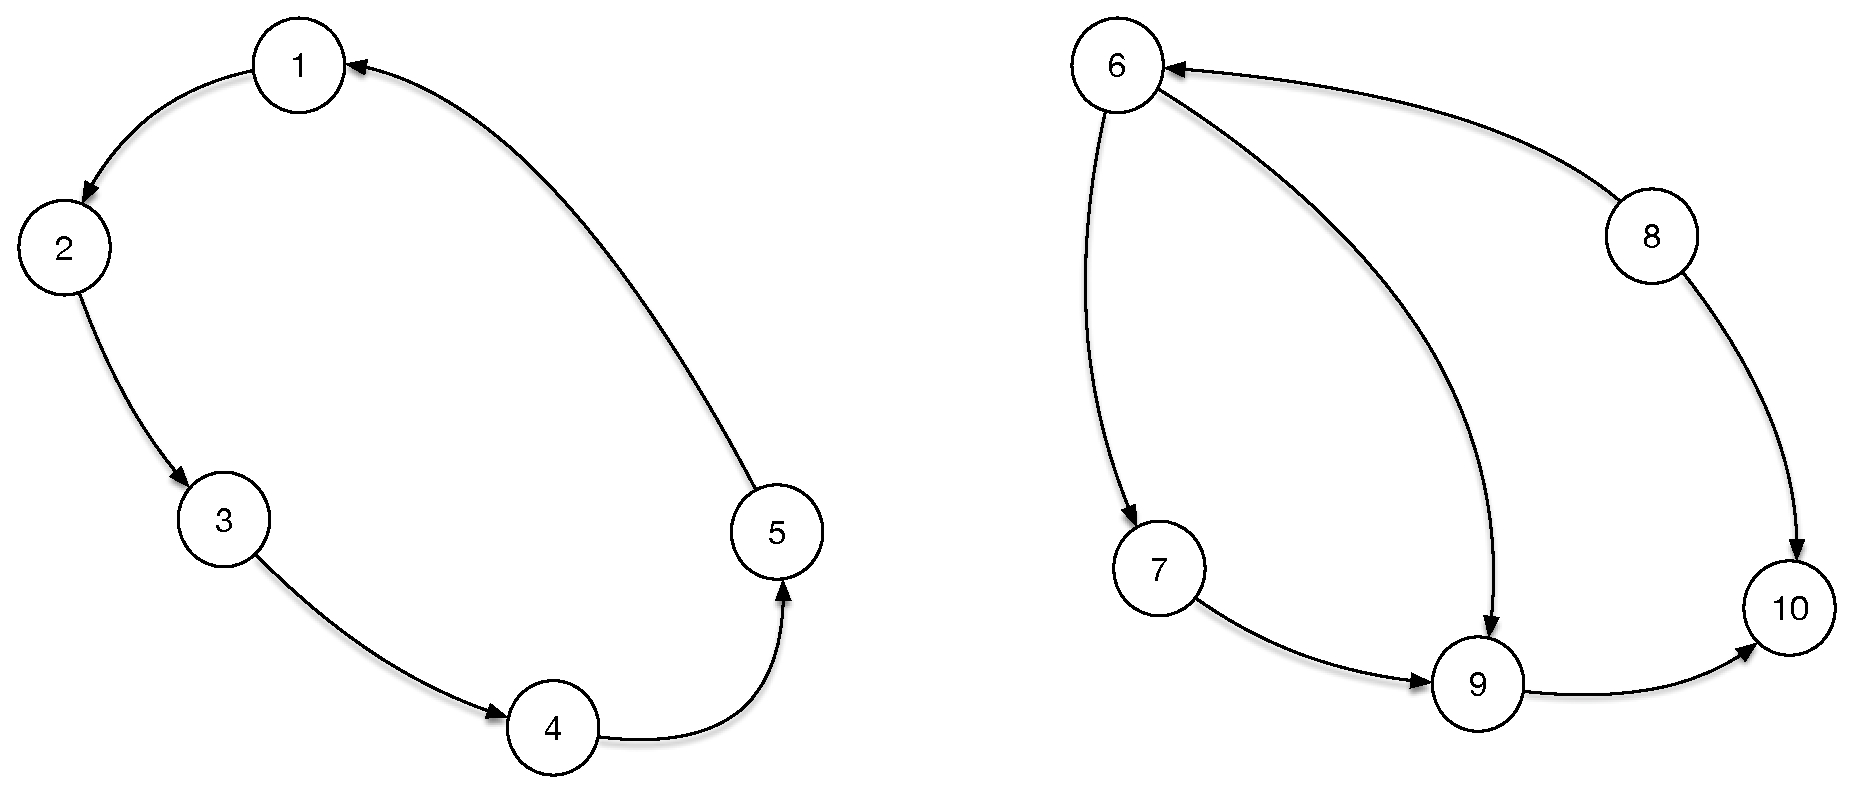
\includegraphics[width=0.7\linewidth]{images/directed_graph_eg}
\end{figure}

\begin{lstlisting}
int main() {
  Graph g;

  Node* node1 = new Node(1);
  Node* node2 = new Node(2);
  Node* node3 = new Node(3);
  Node* node4 = new Node(4);
  Node* node5 = new Node(5);
  Node* node6 = new Node(6);
  Node* node7 = new Node(7);
  Node* node8 = new Node(8);
  Node* node9 = new Node(9);
  Node* node10 = new Node(10);

  g.nodes_.push_back(node1);
  g.nodes_.push_back(node2);
  g.nodes_.push_back(node3);
  g.nodes_.push_back(node4);
  g.nodes_.push_back(node5);
  g.nodes_.push_back(node6);
  g.nodes_.push_back(node7);
  g.nodes_.push_back(node8);
  g.nodes_.push_back(node9);
  g.nodes_.push_back(node10);

  g.Connect(node1, node2);
  g.Connect(node2, node3);
  g.Connect(node3, node4);
  g.Connect(node4, node5);
  g.Connect(node5, node1);
  g.Connect(node6, node7);
  g.Connect(node6, node9);
  g.Connect(node7, node9);
  g.Connect(node8, node6);
  g.Connect(node8, node10);
  g.Connect(node9, node10);

  std::vector<Node*> start_nodes;
  start_nodes.push_back(node1);
  start_nodes.push_back(node8);
  // DFS Recursive: 1 2 3 4 5 8 6 7 9 10
  std::cout << "DFS Recursive: ";
  g.DFSRecursive(start_nodes);
  std::cout << std::endl;
  // DFS Iterative: 8 10 6 9 7 1 2 3 4 5
  std::cout << "DFS Iterative: ";
  g.DFSIterative(start_nodes);
  std::cout << std::endl;
  // BFS: 1 8 2 6 10 3 7 9 4 5
  std::cout << "BFS: ";
  g.BFS(start_nodes);
  std::cout << std::endl;

  // IsCyclicWithoutPruning: True
  std::cout << "IsCyclic: ";
  if (g.IsCyclicWithoutPruining()) {
    std::cout << "True" << std::endl;
  } else {
    std::cout << "False" << std::endl;
  }

  // IsCyclic: True
  std::cout << "IsCyclic: ";
  if (g.IsCyclic()) {
    std::cout << "True" << std::endl;
  } else {
    std::cout << "False" << std::endl;
  }

  return 0;
}
\end{lstlisting}

\subsection{Undirected Graph}
\subsubsection{Data Structures Interfaces}
\begin{lstlisting}
class Node {
 public:
	Node(int val) : val(val) {}
	
	int val;
	std::vector<Edge*> edges_;
};

class Edge {
 public:
	Edge(Node* x, Node* y) : x_(x), y_(y) {}
	
	Node* x_;
	Node* y_;
};

class Graph {
 public:
  Graph() = default;

  void DFSRecursive(std::vector<Node*>& start_nodes);
  void DFSVisit(Node* node, std::unordered_set<Node*>& visited);
  void DFSIterative(std::vector<Node*>& start_nodes);
  void BFS(std::vector<Node*>& start_nodes);

  void Connect(Node* x, Node* y);

  std::vector<Node*> nodes_;
  std::vector<Edge*> edges_;
};
\end{lstlisting}
\subsubsection{DFS - Recursive}
\begin{lstlisting}
void Graph::DFSRecursive(std::vector<Node*>& start_nodes) {
  // we can guarantee visited vector is always up to date because it is passed by reference
  std::unordered_set<Node*> visited;
  for (auto node : start_nodes) {
    if (visited.find(node) == visited.end()) { DFSVisit(node, visited); }
  }
}

void Graph::DFSVisit(Node* node, std::unordered_set<Node*>& visited) {
  if (!node) { return; }
  // handle the node, e.g., print it
  std::cout << node->val << " ";
  visited.insert(node);
  // for each neighbor
  for (auto edge : node->edges_) {
    Node* neighbor = edge->x_ == node ? edge->y_ : edge->x_;
    if (visited.find(neighbor) == visited.end()) { DFSVisit(neighbor, visited); }
  }
}
\end{lstlisting}

\subsubsection{DFS - Iterative}
\begin{lstlisting}
void Graph::DFSIterative(std::vector<Node*>& start_nodes) {
  std::stack<Node*> stk;
  std::unordered_set<Node*> visited;
  for (auto node : start_nodes) {
    stk.push(node);
    visited.insert(node);
  }
  while (!stk.empty()) {
    Node* top = stk.top();
    stk.pop();
    // handle the node, e.g., print it
    std::cout << top->val << " ";
    // for each neighbor
    for (auto edge : top->edges_) {
      Node* neighbor = edge->x_ == top ? edge->y_ : edge->x_;
      if (visited.find(neighbor) == visited.end()) {
        stk.push(neighbor);
        visited.insert(neighbor);
      }
    }
  }
}
\end{lstlisting}

\subsubsection{BFS}
\begin{lstlisting}
void Graph::BFS(std::vector<Node*>& start_nodes) {
  std::queue<Node*> q;
  std::unordered_set<Node*> visited;
  for (auto node : start_nodes) {
    q.push(node);
    visited.insert(node);
  }
  while (!q.empty()) {
    Node* front = q.front();
    q.pop();
    // handle the node, e.g., print it
    std::cout << front->val << " ";
    // for each neighbor
    for (auto edge : front->edges_) {
      Node* neighbor = edge->x_ == front ? edge->y_ : edge->x_;
      if (visited.find(neighbor) == visited.end()) {
        q.push(neighbor);
        visited.insert(neighbor);
      }
    }
  }
}
\end{lstlisting}

\subsubsection{Example}
\begin{figure}[H]
\centering
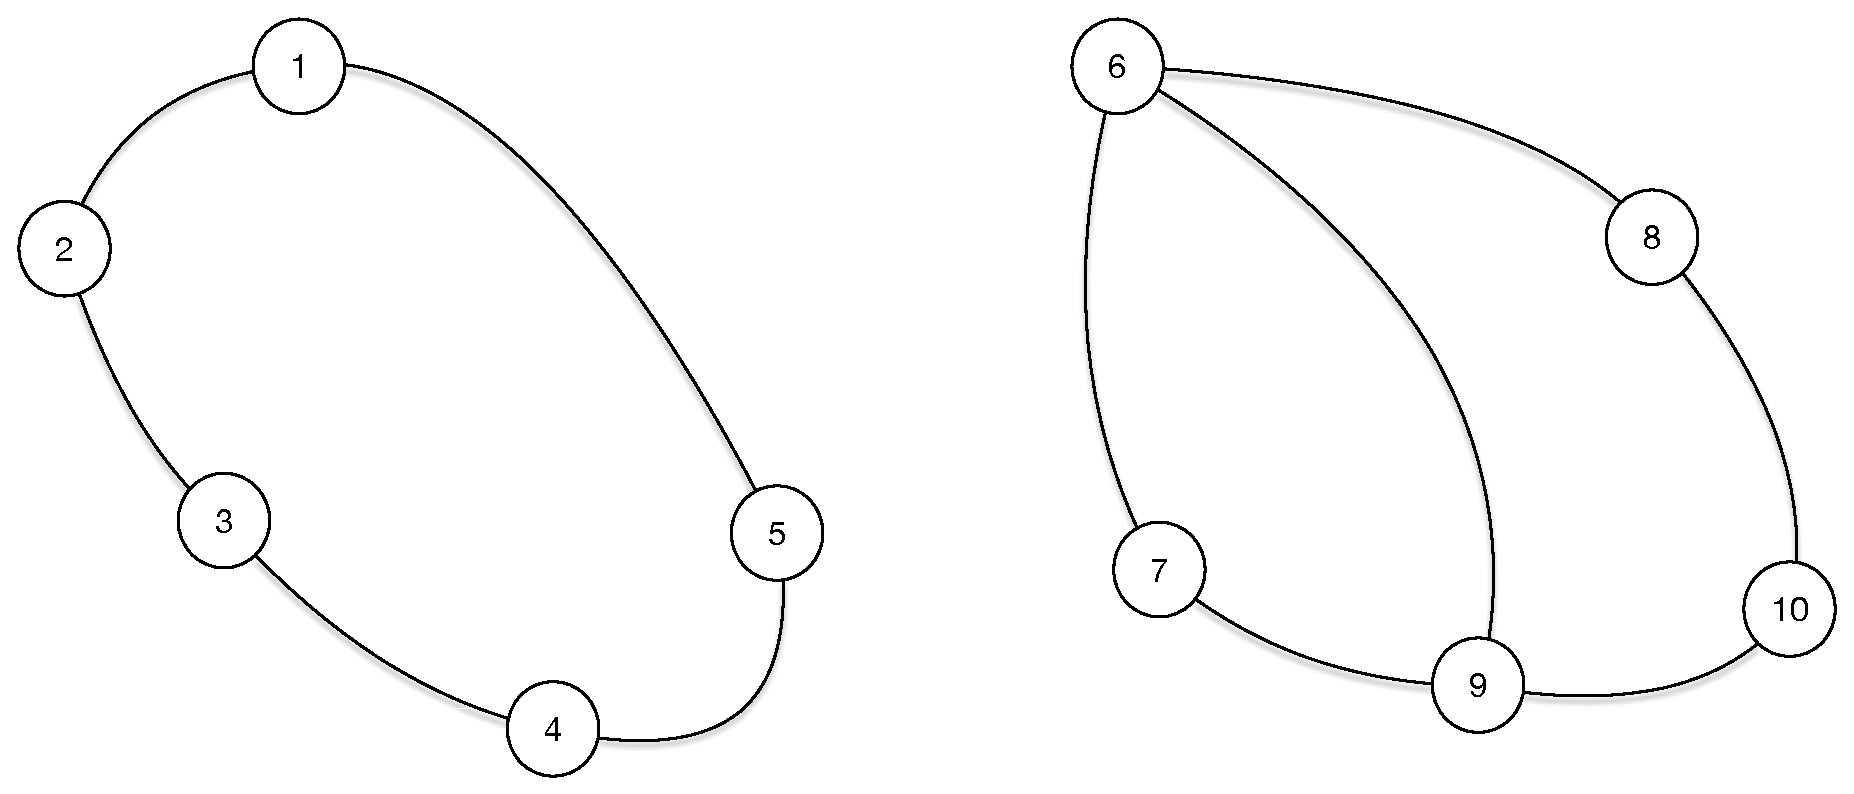
\includegraphics[width=0.7\linewidth]{images/undirected_graph_eg}
\end{figure}
\begin{lstlisting}
int main() {
  Graph g;

  Node* node1 = new Node(1);
  Node* node2 = new Node(2);
  Node* node3 = new Node(3);
  Node* node4 = new Node(4);
  Node* node5 = new Node(5);
  Node* node6 = new Node(6);
  Node* node7 = new Node(7);
  Node* node8 = new Node(8);
  Node* node9 = new Node(9);
  Node* node10 = new Node(10);

  g.nodes_.push_back(node1);
  g.nodes_.push_back(node2);
  g.nodes_.push_back(node3);
  g.nodes_.push_back(node4);
  g.nodes_.push_back(node5);
  g.nodes_.push_back(node6);
  g.nodes_.push_back(node7);
  g.nodes_.push_back(node8);
  g.nodes_.push_back(node9);
  g.nodes_.push_back(node10);

  g.Connect(node1, node2);
  g.Connect(node2, node3);
  g.Connect(node3, node4);
  g.Connect(node4, node5);
  g.Connect(node5, node1);
  g.Connect(node6, node7);
  g.Connect(node6, node9);
  g.Connect(node7, node9);
  g.Connect(node8, node6);
  g.Connect(node8, node10);
  g.Connect(node9, node10);

  std::vector<Node*> start_nodes;
  start_nodes.push_back(node1);
  start_nodes.push_back(node6);
  // DFS Recursive: 1 2 3 4 5 6 7 9 10 8
  std::cout << "DFS Recursive: ";
  g.DFSRecursive(start_nodes);
  std::cout << std::endl;
  // DFS Iterative : 6 8 10 9 7 1 5 4 3 2
  std::cout << "DFS Iterative : ";
  g.DFSIterative(start_nodes);
  std::cout << std::endl;
  // BFS: 1 6 2 5 7 9 8 3 4 10
  std::cout << "BFS: ";
  g.BFS(start_nodes);
  std::cout << std::endl;

  return 0;
}
\end{lstlisting}

\section{Graph (Adjacency List)}
This section explores the implementation of graphs using {\color{blue}{adjacency list}}.\\

It's important to note that ``adjacency list" is a broad term. Beyond just {\color{blue}{lists}}, various {\color{blue}{containers}} can be utilized for storing adjacent nodes. Here, we employ {\colorbox{CodeBackground}{\lstinline|std::vector|}} for this purpose. \\

A distinctive feature of the adjacency list approach is the {\color{blue}{implicit edge representation}}. In this implementation, {\color{blue}{edges}} are not stored as separate entities; rather, they are implied through the relationship between nodes. This simplification sometimes leads to more concise and readable code. \\

However, this method's major drawback is also the lack of explicit edge entities. Because of that, adding extra attributes, like weights, to edges isn't straightforward. For applications requiring such detailed edge information, an alternative approach, such as the {\color{blue}{universal implementation}} or an {\color{blue}{adjacency matrix}}, might be more appropriate.

\subsection{Directed Graph}
\subsubsection{Data Structures Interfaces}
\begin{lstlisting}
class Node {
 public:
  Node() = default;
  Node(int val) : val_(val) {}

  int val_;
  std::vector<Node*> neighbors;
};

void Connect(Node* src, Node* dst) { src->neighbors.push_back(dst); }
\end{lstlisting}
\subsubsection{DFS}
\begin{lstlisting}
void DFS(std::vector<Node*>& start_nodes) {
  // we can guarantee visited vector is always up to date because it is passed by reference
  std::unordered_set<Node*> visited;
  for (auto node : start_nodes) {
    if (visited.find(node) == visited.end()) { DFSVisit(node, visited); }
  }
}

void DFSVisit(Node* node, std::unordered_set<Node*>& visited) {
  if (!node) { return; }
  // handle the node, e.g., print it
  std::cout << node->val_ << " ";
  visited.insert(node);
  // for each neighbor
  for (Node* neighbor : node->neighbors) {
    if (visited.find(neighbor) == visited.end()) { DFSVisit(neighbor, visited); }
  }
}
\end{lstlisting}
\subsubsection{BFS}
\begin{lstlisting}
void BFS(std::vector<Node*>& start_nodes) {
  std::queue<Node*> q;
  std::unordered_set<Node*> visited;
  for (auto node : start_nodes) {
    q.push(node);
    visited.insert(node);
  }
  while (!q.empty()) {
    Node* front = q.front();
    q.pop();
    // handle the node, e.g., print it
    std::cout << front->val_ << " ";
    // for each neighbor
    for (Node* neighbor : front->neighbors) {
      if (visited.find(neighbor) == visited.end()) {
        q.push(neighbor);
        visited.insert(neighbor);
      }
    }
  }
}
\end{lstlisting}

\subsubsection{Detect Cycles}
\begin{lstlisting}
bool IsAcyclic(std::vector<Node*>& graph) {
  std::unordered_set<Node*> path;
  // nodes that have been explored and not in any cycle
  std::unordered_set<Node*> visited;
  for (Node* node : graph) {
    if (DetectCycleFromNode(node, path, visited)) { return true; }
  }
  return false;
}

bool DetectCycleFromNode(Node* node, std::unordered_set<Node*>& path,
                         std::unordered_set<Node*>& visited) {
  // edge case - null node
  if (!node) { return false; }
  // base case - cycle detected
  if (path.find(node) != path.end()) { return true; }
  // pruning - visited node
  if (visited.find(node) != visited.end()) { return false; }
  path.insert(node);
  visited.insert(node);
  for (Node* neighbor : node->neighbors) {
    if (DetectCycleFromNode(neighbor, visited, path)) { return true; }
  }
  path.erase(node);
  return false;
}
\end{lstlisting}

\subsubsection{Example}
\begin{figure}[H]
\centering
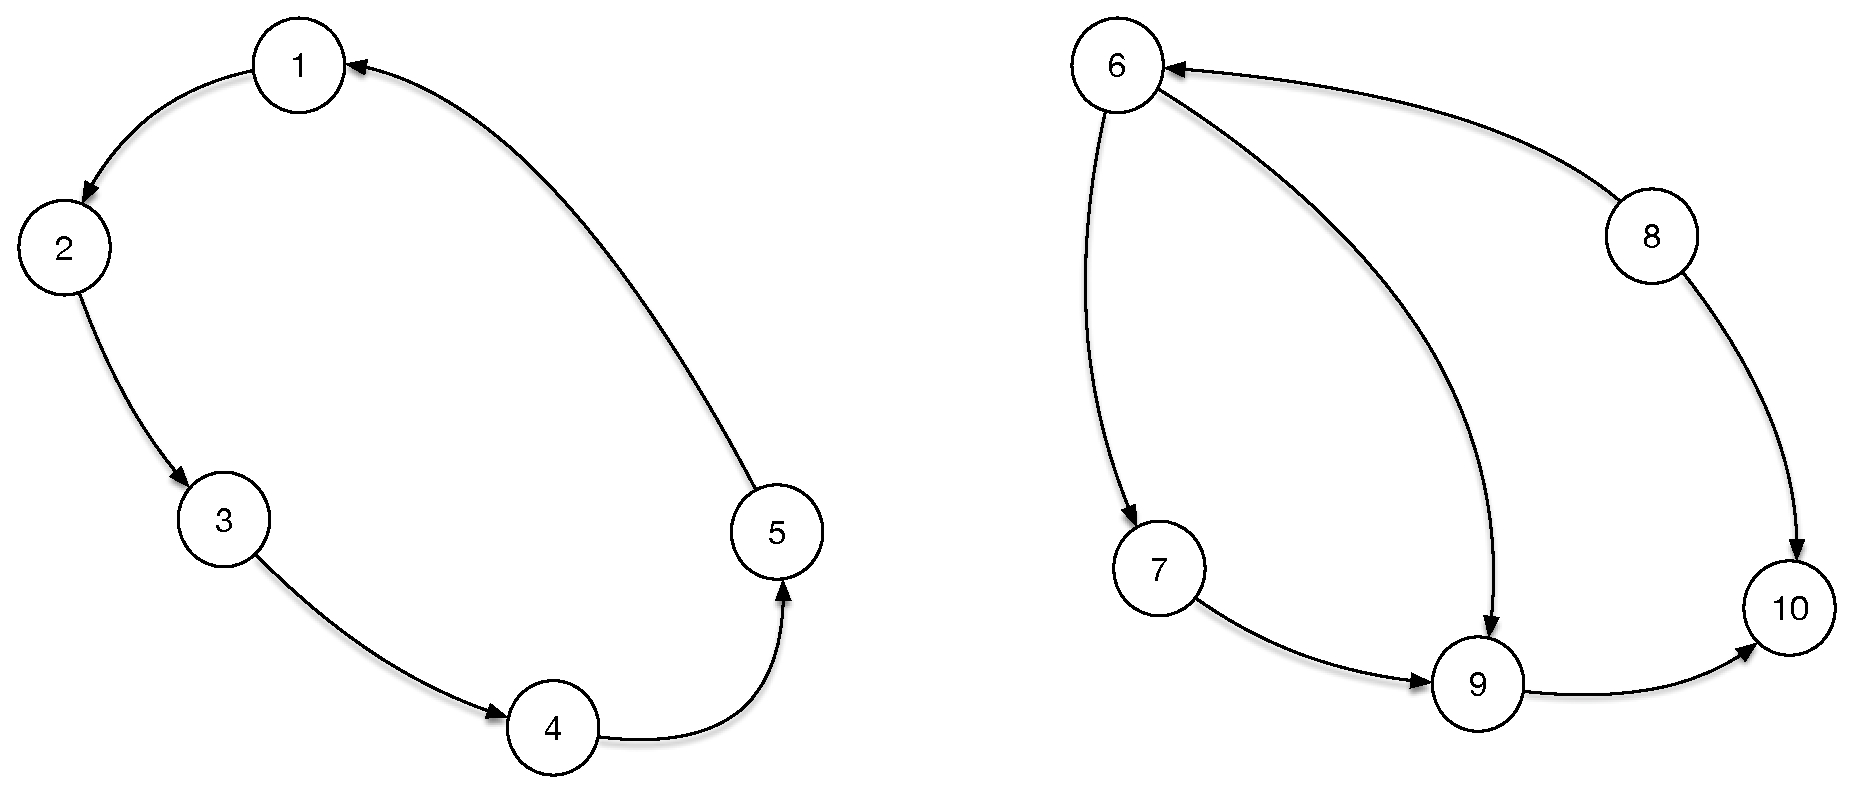
\includegraphics[width=0.7\linewidth]{images/directed_graph_eg}
\end{figure}

\begin{lstlisting}
int main() {
  std::vector<Node*> graph;
  for (int i = 1; i <= 10; ++i) { graph.push_back(new Node(i)); }
  Connect(graph[0], graph[1]);
  Connect(graph[1], graph[2]);
  Connect(graph[2], graph[3]);
  Connect(graph[3], graph[4]);
  Connect(graph[4], graph[0]);
  Connect(graph[5], graph[6]);
  Connect(graph[5], graph[8]);
  Connect(graph[6], graph[8]);
  Connect(graph[7], graph[5]);
  Connect(graph[7], graph[9]);
  Connect(graph[8], graph[9]);

  std::vector<Node*> start_nodes;
  start_nodes.push_back(graph[0]);
  start_nodes.push_back(graph[7]);
  // DFS : 1 2 3 4 5 8 6 7 9 10
  std::cout << "DFS: " << std::endl;
  DFS(start_nodes);
  std::cout << std::endl;
  // BFS: 1 8 2 6 10 3 7 9 4 5
  std::cout << "BFS: " << std::endl;
  BFS(start_nodes);
  std::cout << std::endl;

  // IsAcyclic: True
  std::cout << "IsAcyclic: ";
  if (IsAcyclic(graph)) {
    std::cout << "True" << std::endl;
  } else {
    std::cout << "False" << std::endl;
  }

  return 0;
}
\end{lstlisting}

\subsection{Undirected Graph}
In {\color{blue}{adjacency list}}, the most fundamental difference between {\color{blue}{undirected graph}} and {\color{blue}{directed graph}} lies in the {\colorbox{CodeBackground}{\lstinline|Connect|}} function; everything else is the same.
\begin{lstlisting}
// directed graph
void Connect(Node* src, Node* dst) { 
	src->neighbors.push_back(dst);
}

// undirected graph
void Connect(Node* src, Node* dst) {
	src->neighbors.push_back(dst);
	dst->neighbors.push_back(src);
}
\end{lstlisting}

\subsubsection{Data Structures Interfaces}
\begin{lstlisting}
class Node {
	public:
	Node() = default;
	Node(int val) : val_(val) {}
	
	int val_;
	std::vector<Node*> neighbors;
};

void Connect(Node* src, Node* dst) {
	src->neighbors.push_back(dst);
	dst->neighbors.push_back(src);
}
\end{lstlisting}
\subsubsection{DFS}
\begin{lstlisting}
void DFS(std::vector<Node*>& start_nodes) {
  // we can guarantee visited vector is always up to date because it is passed by reference
  std::unordered_set<Node*> visited;
  for (auto node : start_nodes) {
    if (visited.find(node) == visited.end()) { DFSVisit(node, visited); }
  }
}

void DFSVisit(Node* node, std::unordered_set<Node*>& visited) {
  if (!node) { return; }
  // handle the node, e.g., print it
  std::cout << node->val_ << " ";
  visited.insert(node);
  // for each neighbor
  for (Node* neighbor : node->neighbors) {
    if (visited.find(neighbor) == visited.end()) { DFSVisit(neighbor, visited); }
  }
}
\end{lstlisting}
\subsubsection{BFS}
\begin{lstlisting}
void BFS(std::vector<Node*>& start_nodes) {
  std::queue<Node*> q;
  std::unordered_set<Node*> visited;
  for (auto node : start_nodes) {
    q.push(node);
    visited.insert(node);
  }
  while (!q.empty()) {
    Node* front = q.front();
    q.pop();
    // handle the node, e.g., print it
    std::cout << front->val_ << " ";
    // for each neighbor
    for (Node* neighbor : front->neighbors) {
      if (visited.find(neighbor) == visited.end()) {
        q.push(neighbor);
        visited.insert(neighbor);
      }
    }
  }
}
\end{lstlisting}

\subsubsection{Example}
\begin{figure}[H]
\centering
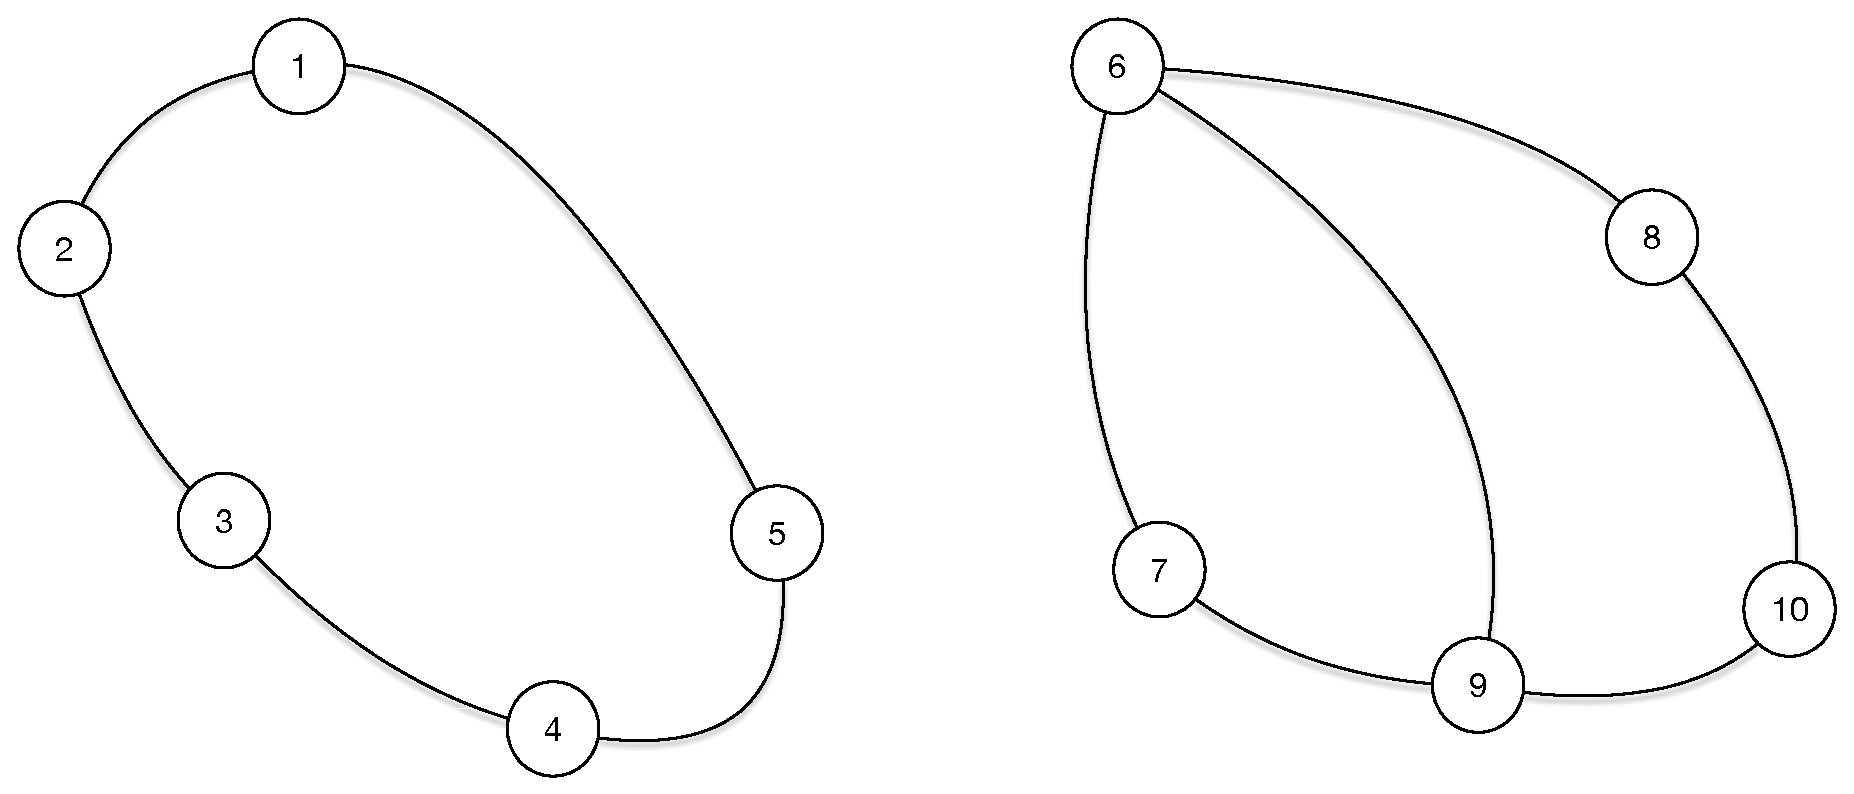
\includegraphics[width=0.7\linewidth]{images/undirected_graph_eg}
\end{figure}

\begin{lstlisting}
int main() {
  std::vector<Node*> graph;
  for (int i = 1; i <= 10; ++i) { graph.push_back(new Node(i)); }
  Connect(graph[0], graph[1]);
  Connect(graph[1], graph[2]);
  Connect(graph[2], graph[3]);
  Connect(graph[3], graph[4]);
  Connect(graph[4], graph[0]);
  Connect(graph[5], graph[6]);
  Connect(graph[5], graph[8]);
  Connect(graph[6], graph[8]);
  Connect(graph[7], graph[5]);
  Connect(graph[7], graph[9]);
  Connect(graph[8], graph[9]);

  std::vector<Node*> start_nodes;
  start_nodes.push_back(graph[0]);
  start_nodes.push_back(graph[7]);
  // DFS: 1 2 3 4 5 8 6 7 9 10
  std::cout << "DFS: " << std::endl;
  DFS(start_nodes);
  std::cout << std::endl;
  // BFS: 1 8 2 5 6 10 3 4 7 9
  std::cout << "BFS: " << std::endl;
  BFS(start_nodes);
  std::cout << std::endl;

  return 0;
}
\end{lstlisting}

\section{Graph (Adjacency Matrix)}
This section explores the implementation of graphs using {\color{blue}{adjacency matrix}}.\\

A distinctive feature of the adjacency matrix approach is the {\color{blue}{implicit node representation}}. In this implementation, {\color{blue}{nodes}} are not stored as separate entities; rather, they are just indices. The matrix entries represent {\color{blue}{edges}}, e.g., with weights assigned to these edges here.  This simplification sometimes leads to more concise and readable code. \\

However, this method's major drawback is also the lack of explicit node entities. Because of that, adding extra attributes, like weights, to nodes isn't straightforward. For applications requiring such detailed node information, an alternative approach, such as the {\color{blue}{universal implementation}} or an {\color{blue}{adjacency list}}, might be more appropriate.

\subsection{Directed Graph}
\subsubsection{Data Structures Interfaces}
\begin{lstlisting}
// representation of graph
std::vector<std::vector<int>> graph(num_nodes, std::vector<int>(num_nodes, 0));

// weight = 0 means no edge
// o.w., weight is always positive
void Connect(std::vector<std::vector<int>>& graph, int src, int dst, int w) {
  graph[src][dst] = w;
}
\end{lstlisting}
\subsubsection{DFS}
\begin{lstlisting}
void DFS(std::vector<std::vector<int>>& graph, std::vector<int>& start_nodes) {
  // we can guarantee visited vector is always up to date because it is passed by reference
  std::vector<bool> visited(graph.size(), false);
  for (auto node : start_nodes) {
    if (!visited[node]) { DFSVisit(graph, node, visited); }
  }
}

void DFSVisit(std::vector<std::vector<int>>& graph, int node, std::vector<bool>& visited) {
  // handle the node, e.g., print it
  std::cout << node + 1 << " ";
  visited[node] = true;
  // for each neighbor
  for (int i = 0; i < graph.size(); ++i) {
    if (graph[node][i] != 0 && !visited[i]) { DFSVisit(graph, i, visited); }
  }
}
\end{lstlisting}
\subsubsection{BFS}
\begin{lstlisting}
void BFS(std::vector<std::vector<int>>& graph, std::vector<int>& start_nodes) {
  std::queue<int> q;
  std::vector<bool> visited(graph.size(), false);
  for (auto node : start_nodes) {
    q.push(node);
    visited[node] = true;
  }
  while (!q.empty()) {
    int front = q.front();
    q.pop();
    // handle the node, e.g., print it
    std::cout << front + 1 << " ";
    // for each neighbor
    for (int i = 0; i < graph.size(); ++i) {
      if (graph[front][i] != 0 && !visited[i]) {
        q.push(i);
        visited[i] = true;
      }
    }
  }
}
\end{lstlisting}

\subsubsection{Detect Cycles}
\begin{lstlisting}
bool IsAcyclic(std::vector<std::vector<int>> graph) {
  std::vector<bool> path(graph.size(), false);
  // nodes that have been explored and not in any cycle
  std::vector<bool> visited(graph.size(), false);
  for (int i = 0; i < graph.size(); ++i) {
    if (DetectCycleFromNode(graph, i, visited, path)) { return true; }
  }
  return false;
}

bool DetectCycleFromNode(std::vector<std::vector<int>>& graph, int node,
                         std::vector<bool>& visited, std::vector<bool>& path) {
  // base case - null node
  if (node < 0 || node >= graph.size()) { return false; }
  // base case - cycle detected
  if (path[node]) { return true; }
  // pruning - visited node
  if (visited[node]) { return false; }
  path[node] = true;
  visited[node] = true;
  for (int i = 0; i < graph.size(); ++i) {
    if (graph[node][i] != 0) {
      if (DetectCycleFromNode(graph, i, visited, path)) { return true; }
    }
  }
  path[node] = false;
  return false;
}
\end{lstlisting}

\subsubsection{Example}
\begin{figure}[H]
\centering
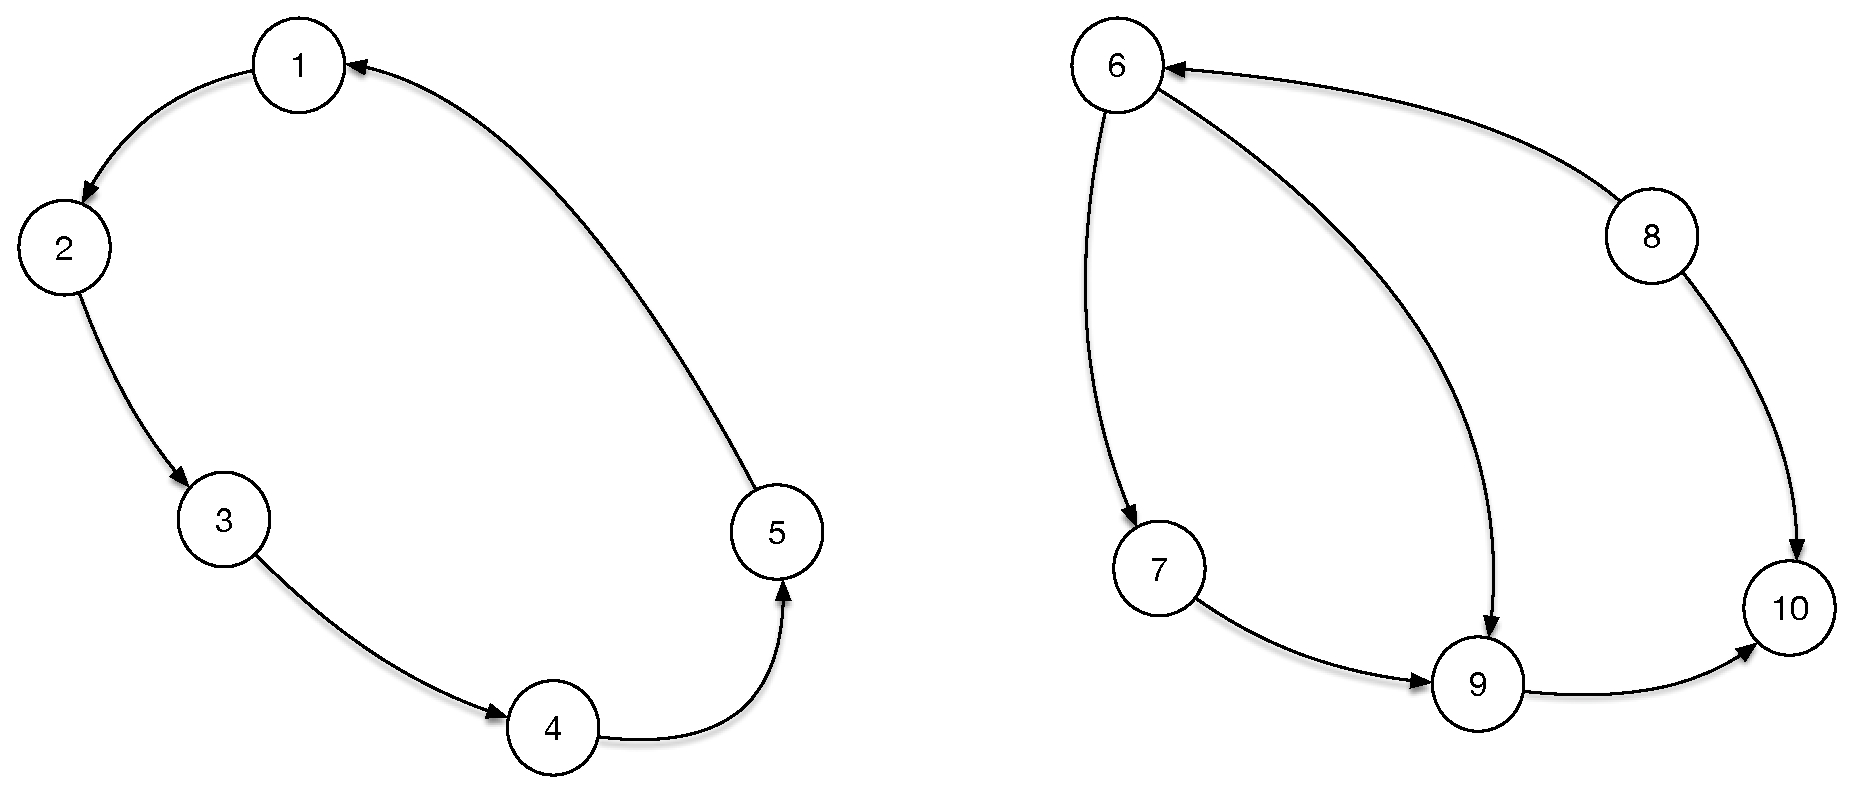
\includegraphics[width=0.7\linewidth]{images/directed_graph_eg}
\end{figure}

\begin{lstlisting}
int main() {
  std::vector<std::vector<int>> graph(10, std::vector<int>(10, 0));

  Connect(graph, 0, 1, 1);
  Connect(graph, 1, 2, 1);
  Connect(graph, 2, 3, 1);
  Connect(graph, 3, 4, 1);
  Connect(graph, 4, 0, 1);
  Connect(graph, 5, 6, 1);
  Connect(graph, 5, 8, 1);
  Connect(graph, 6, 8, 1);
  Connect(graph, 7, 5, 1);
  Connect(graph, 7, 9, 1);
  Connect(graph, 8, 9, 1);

  std::vector<int> start_nodes = {0, 7};
  // DFS: 1 2 3 4 5 8 6 7 9 10
  std::cout << "DFS: ";
  DFS(graph, start_nodes);
  std::cout << std::endl;
  // BFS: 1 8 2 6 10 3 7 9 4 5
  std::cout << "BFS: ";
  BFS(graph, start_nodes);
  std::cout << std::endl;

  // IsCyclic: True
  std::cout << "IsCyclic: ";
  if (IsAcyclic(graph)) {
    std::cout << "True" << std::endl;
  } else {
    std::cout << "False" << std::endl;
  }

  return 0;
}
\end{lstlisting}

\subsection{Undirected Graph}
In {\color{blue}{adjacency matrix}}, the most fundamental difference between {\color{blue}{undirected graph}} and {\color{blue}{directed graph}} lies in the {\colorbox{CodeBackground}{\lstinline|Connect|}} function; everything else is the same.
\begin{lstlisting}
// directed graph
void Connect(std::vector<std::vector<int>>& graph, int src, int dst, int w) {
  graph[src][dst] = w;
}

// undirected graph
void Connect(std::vector<std::vector<int>>& graph, int x, int y, int w) {
	graph[x][y] = w;
	graph[y][x] = w;
}
\end{lstlisting}
\subsubsection{Data Structures Interfaces}
\begin{lstlisting}
// representation of graph
std::vector<std::vector<int>> graph(num_nodes, std::vector<int>(num_nodes, 0));

// weight = 0 means no edge
// o.w., weight is always positive
void Connect(std::vector<std::vector<int>>& graph, int x, int y, int w) {
	graph[x][y] = w;
	graph[y][x] = w;
}
\end{lstlisting}

\subsubsection{DFS}
\begin{lstlisting}
void DFS(std::vector<std::vector<int>>& graph, std::vector<int>& start_nodes) {
  // we can guarantee visited vector is always up to date because it is passed by reference
  std::vector<bool> visited(graph.size(), false);
  for (auto node : start_nodes) {
    if (!visited[node]) { DFSVisit(graph, node, visited); }
  }
}

void DFSVisit(std::vector<std::vector<int>>& graph, int node, std::vector<bool>& visited) {
  // handle the node, e.g., print it
  std::cout << node + 1 << " ";
  visited[node] = true;
  // for each neighbor
  for (int i = 0; i < graph.size(); ++i) {
    if (graph[node][i] != 0 && !visited[i]) { DFSVisit(graph, i, visited); }
  }
}
\end{lstlisting}
\subsubsection{BFS}
\begin{lstlisting}
void BFS(std::vector<std::vector<int>>& graph, std::vector<int>& start_nodes) {
  std::queue<int> q;
  std::vector<bool> visited(graph.size(), false);
  for (auto node : start_nodes) {
    q.push(node);
    visited[node] = true;
  }
  while (!q.empty()) {
    int front = q.front();
    q.pop();
    // handle the node, e.g., print it
    std::cout << front + 1 << " ";
    // for each neighbor
    for (int i = 0; i < graph.size(); ++i) {
      if (graph[front][i] != 0 && !visited[i]) {
        q.push(i);
        visited[i] = true;
      }
    }
  }
}
\end{lstlisting}

\subsubsection{Example}
\begin{figure}[H]
\centering
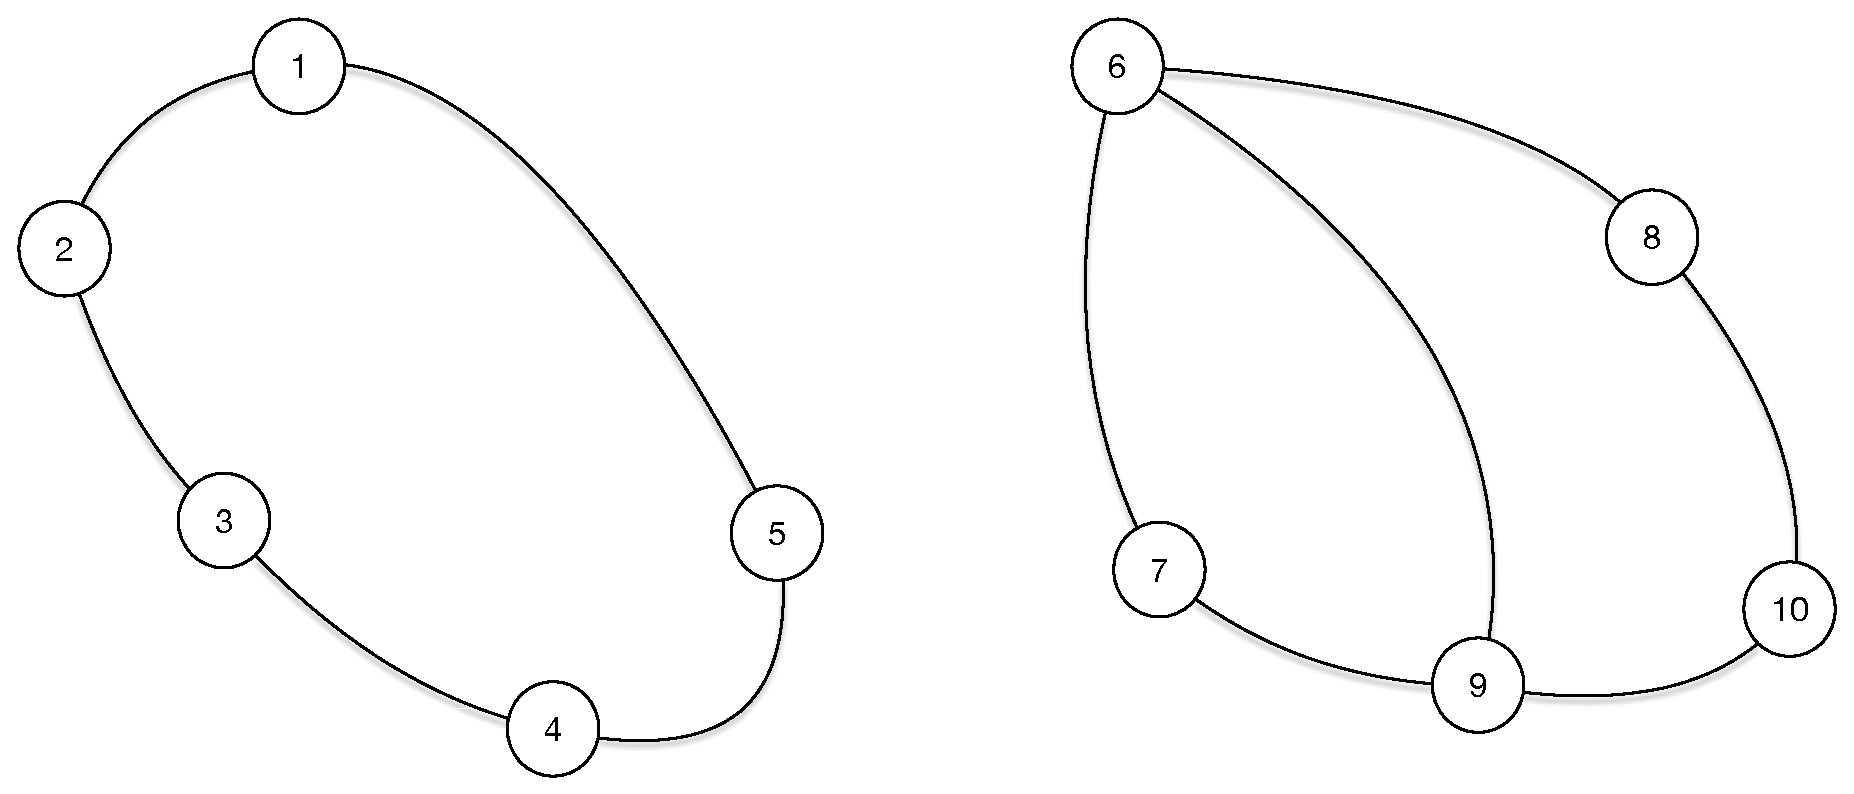
\includegraphics[width=0.7\linewidth]{images/undirected_graph_eg}
\end{figure}

\begin{lstlisting}
int main() {
  std::vector<std::vector<int>> graph(10, std::vector<int>(10, 0));

  Connect(graph, 0, 1, 1);
  Connect(graph, 1, 2, 1);
  Connect(graph, 2, 3, 1);
  Connect(graph, 3, 4, 1);
  Connect(graph, 4, 0, 1);
  Connect(graph, 5, 6, 1);
  Connect(graph, 5, 8, 1);
  Connect(graph, 6, 8, 1);
  Connect(graph, 7, 5, 1);
  Connect(graph, 7, 9, 1);
  Connect(graph, 8, 9, 1);

  std::vector<int> start_nodes = {0, 7};
  // DFS: 1 2 3 4 5 8 6 7 9 10
  std::cout << "DFS: ";
  DFS(graph, start_nodes);
  std::cout << std::endl;
  // BFS: 1 8 2 6 10 3 7 9 4 5
  std::cout << "BFS: ";
  BFS(graph, start_nodes);
  std::cout << std::endl;

  return 0;
}
\end{lstlisting}

\section{Graph (Sparse Adjacency Matrix)}
This section explores the implementation of graphs using {\color{blue}{sparse adjacency matrix}}, which is a variant of the {\color{blue}{adjacency matrix}}.

\subsection{Directed Graph}
\subsubsection{Data Structures Interfaces}
\begin{lstlisting}
// representation of graph
// to make sure that we can get correct graph size by graph.size()
  std::unordered_map<int, std::unordered_map<int, int>> graph = {
      {1, std::unordered_map<int, int>()}, {2, std::unordered_map<int, int>()},
      {3, std::unordered_map<int, int>()}, {4, std::unordered_map<int, int>()},
      {5, std::unordered_map<int, int>()}, {6, std::unordered_map<int, int>()},
      {7, std::unordered_map<int, int>()}, {8, std::unordered_map<int, int>()},
      {9, std::unordered_map<int, int>()}, {10, std::unordered_map<int, int>()}};

void Connect(std::unordered_map<int, std::unordered_map<int, int>>& graph, int src, int dst,
             int w) {
  graph[src][dst] = w;
}
\end{lstlisting}
\subsubsection{DFS}
\begin{lstlisting}
void DFS(std::unordered_map<int, std::unordered_map<int, int>>& graph,
         std::vector<int>& start_nodes) {
  // we can guarantee visited vector is always up to date because it is passed by reference
  std::vector<bool> visited(graph.size(), false);
  for (auto node : start_nodes) {
    if (!visited[node]) { DFSVisit(graph, node, visited); }
  }
}

void DFSVisit(std::unordered_map<int, std::unordered_map<int, int>>& graph, int node,
              std::vector<bool>& visited) {
  // handle the node, e.g., print it
  std::cout << node << " ";
  visited[node] = true;
  // for each neighbor
  for (auto& neighbor : graph[node]) {
    if (!visited[neighbor.first]) { DFSVisit(graph, neighbor.first, visited); }
  }
}
\end{lstlisting}
\subsubsection{BFS}
\begin{lstlisting}
void BFS(std::unordered_map<int, std::unordered_map<int, int>>& graph,
         std::vector<int>& start_nodes) {
  std::queue<int> q;
  std::vector<bool> visited(graph.size(), false);
  for (auto node : start_nodes) {
    q.push(node);
    visited[node] = true;
  }
  while (!q.empty()) {
    int front = q.front();
    q.pop();
    // handle the node, e.g., print it
    std::cout << front << " ";
    // for each neighbor
    for (auto& neighbor : graph[front]) {
      if (!visited[neighbor.first]) {
        q.push(neighbor.first);
        visited[neighbor.first] = true;
      }
    }
  }
}
\end{lstlisting}

\subsubsection{Detect Cycles}
\begin{lstlisting}
bool IsAcyclic(std::unordered_map<int, std::unordered_map<int, int>> graph) {
  std::vector<bool> path(graph.size(), false);
  // nodes that have been explored and not in any cycle
  std::vector<bool> visited(graph.size(), false);
  for (const auto& node : graph) {
    if (DetectCycleFromNode(graph, node.first, visited, path)) { return true; }
  }
  return false;
}

bool DetectCycleFromNode(std::unordered_map<int, std::unordered_map<int, int>>& graph,
                         int node, std::vector<bool>& visited, std::vector<bool>& path) {
  // edge case - null node
  if (node < 0 || node >= graph.size()) { return false; }
  // base case - cycle detected
  if (path[node]) { return true; }
  // pruning - visited node
  if (visited[node]) { return false; }
  path[node] = true;
  visited[node] = true;
  for (auto& neighbor : graph[node]) {
    if (DetectCycleFromNode(graph, neighbor.first, visited, path)) { return true; }
  }
  path[node] = false;
  return false;
}
\end{lstlisting}

\subsubsection{Example}
\begin{figure}[H]
\centering
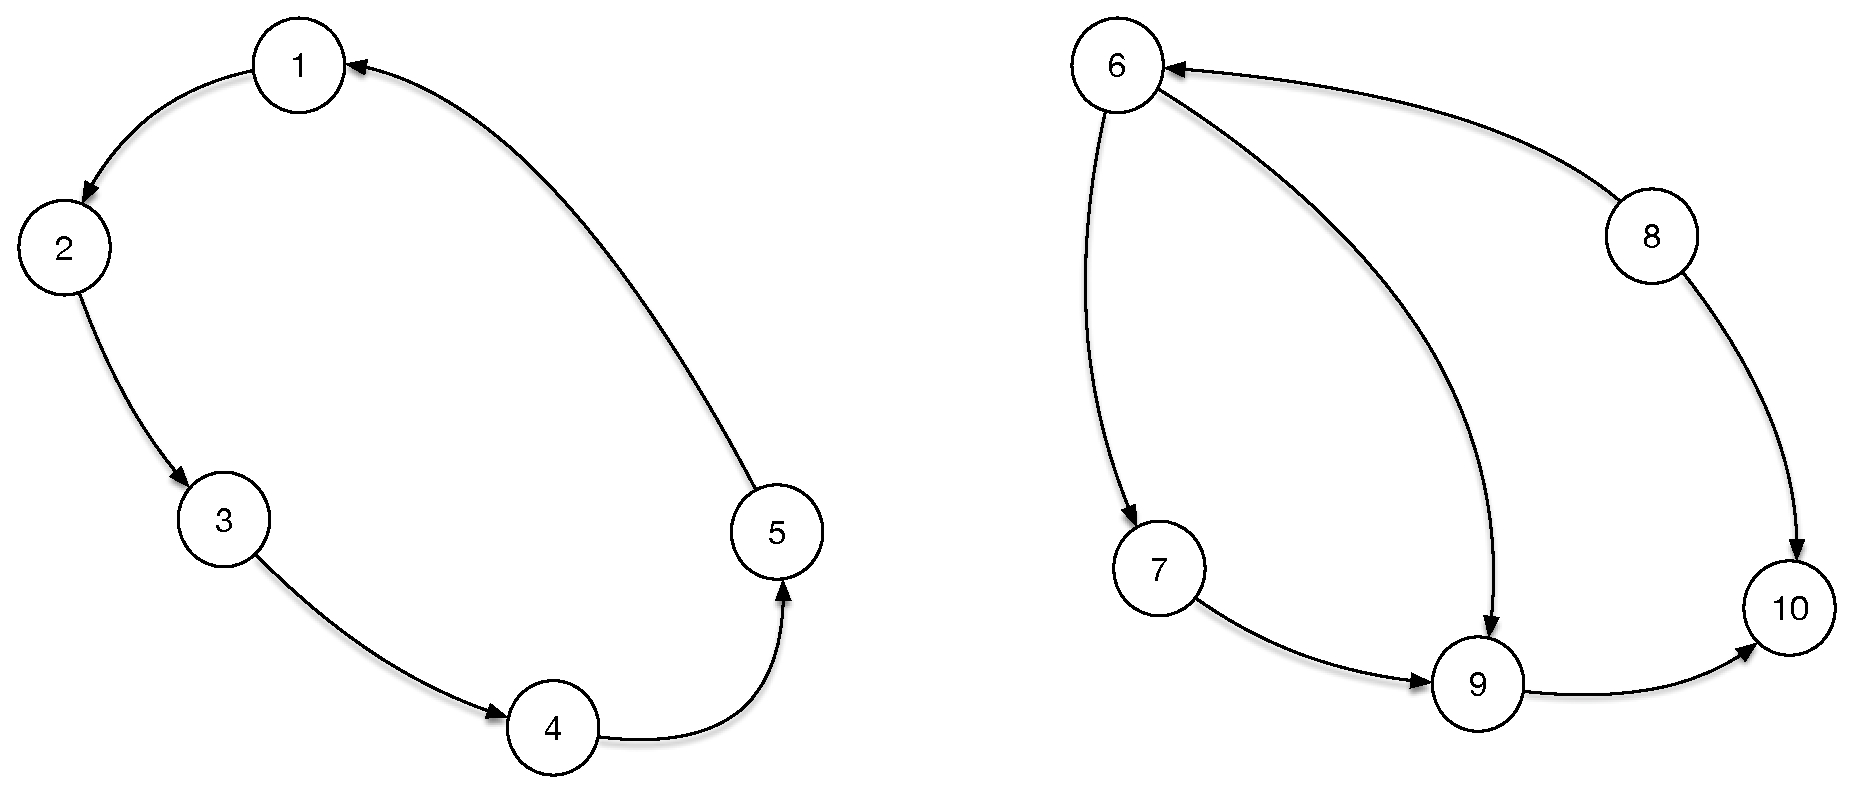
\includegraphics[width=0.7\linewidth]{images/directed_graph_eg}
\end{figure}

\begin{lstlisting}
int main() {
  // to make sure that we can get correct graph size by graph.size()
  std::unordered_map<int, std::unordered_map<int, int>> graph = {
      {1, std::unordered_map<int, int>()}, {2, std::unordered_map<int, int>()},
      {3, std::unordered_map<int, int>()}, {4, std::unordered_map<int, int>()},
      {5, std::unordered_map<int, int>()}, {6, std::unordered_map<int, int>()},
      {7, std::unordered_map<int, int>()}, {8, std::unordered_map<int, int>()},
      {9, std::unordered_map<int, int>()}, {10, std::unordered_map<int, int>()}};

  Connect(graph, 1, 2, 1);
  Connect(graph, 2, 3, 1);
  Connect(graph, 3, 4, 1);
  Connect(graph, 4, 5, 1);
  Connect(graph, 5, 1, 1);
  Connect(graph, 6, 7, 1);
  Connect(graph, 6, 9, 1);
  Connect(graph, 7, 9, 1);
  Connect(graph, 8, 6, 1);
  Connect(graph, 8, 10, 1);
  Connect(graph, 9, 10, 1);

  std::vector<int> start_nodes = {1, 8};
  // DFS: 1 2 3 4 5 8 10 6 9 7
  std::cout << "DFS: ";
  DFS(graph, start_nodes);
  std::cout << std::endl;
  // BFS: 1 8 2 10 6 3 9 7 4 5
  std::cout << "BFS: ";
  BFS(graph, start_nodes);
  std::cout << std::endl;

  // IsCyclic: True
  std::cout << "IsCyclic: ";
  if (IsAcyclic(graph)) {
    std::cout << "True" << std::endl;
  } else {
    std::cout << "False" << std::endl;
  }

  return 0;
}
\end{lstlisting}

\subsection{Undirected Graph}
In {\color{blue}{sparse adjacency matrix}}, the most fundamental difference between {\color{blue}{undirected graph}} and {\color{blue}{directed graph}} lies in the {\colorbox{CodeBackground}{\lstinline|Connect|}} function; everything else is the same.

\begin{lstlisting}
// directed graph
void Connect(std::unordered_map<int, std::unordered_map<int, int>>& graph, int src, int dst,
             int w) {
  graph[src][dst] = w;
}

// undirected graph
void Connect(std::vector<std::vector<int>>& graph, int x, int y, int w) {
	graph[x][y] = w;
	graph[y][x] = w;
}
\end{lstlisting}
\subsubsection{Data Structures Interfaces}
\begin{lstlisting}
// representation of graph
// to make sure that we can get correct graph size by graph.size()
  std::unordered_map<int, std::unordered_map<int, int>> graph = {
      {1, std::unordered_map<int, int>()}, {2, std::unordered_map<int, int>()},
      {3, std::unordered_map<int, int>()}, {4, std::unordered_map<int, int>()},
      {5, std::unordered_map<int, int>()}, {6, std::unordered_map<int, int>()},
      {7, std::unordered_map<int, int>()}, {8, std::unordered_map<int, int>()},
      {9, std::unordered_map<int, int>()}, {10, std::unordered_map<int, int>()}};
	
void Connect(std::unordered_map<int, std::unordered_map<int, int>>& graph, int x, int y,
             int w) {
  graph[x][y] = w;
  graph[y][x] = w;
}
\end{lstlisting}
\subsubsection{DFS}
\begin{lstlisting}
void DFS(std::unordered_map<int, std::unordered_map<int, int>>& graph,
         std::vector<int>& start_nodes) {
  // we can guarantee visited vector is always up to date because it is passed by reference
  std::vector<bool> visited(graph.size(), false);
  for (auto node : start_nodes) {
    if (!visited[node]) { DFSVisit(graph, node, visited); }
  }
}

void DFSVisit(std::unordered_map<int, std::unordered_map<int, int>>& graph, int node,
              std::vector<bool>& visited) {
  // handle the node, e.g., print it
  std::cout << node << " ";
  visited[node] = true;
  // for each neighbor
  for (auto& neighbor : graph[node]) {
    if (!visited[neighbor.first]) { DFSVisit(graph, neighbor.first, visited); }
  }
}
\end{lstlisting}
\subsubsection{BFS}
\begin{lstlisting}
void BFS(std::unordered_map<int, std::unordered_map<int, int>>& graph,
         std::vector<int>& start_nodes) {
  std::queue<int> q;
  std::vector<bool> visited(graph.size(), false);
  for (auto node : start_nodes) {
    q.push(node);
    visited[node] = true;
  }
  while (!q.empty()) {
    int front = q.front();
    q.pop();
    // handle the node, e.g., print it
    std::cout << front << " ";
    // for each neighbor
    for (auto& neighbor : graph[front]) {
      if (!visited[neighbor.first]) {
        q.push(neighbor.first);
        visited[neighbor.first] = true;
      }
    }
  }
}
\end{lstlisting}

\subsubsection{Example}
\begin{figure}[H]
\centering
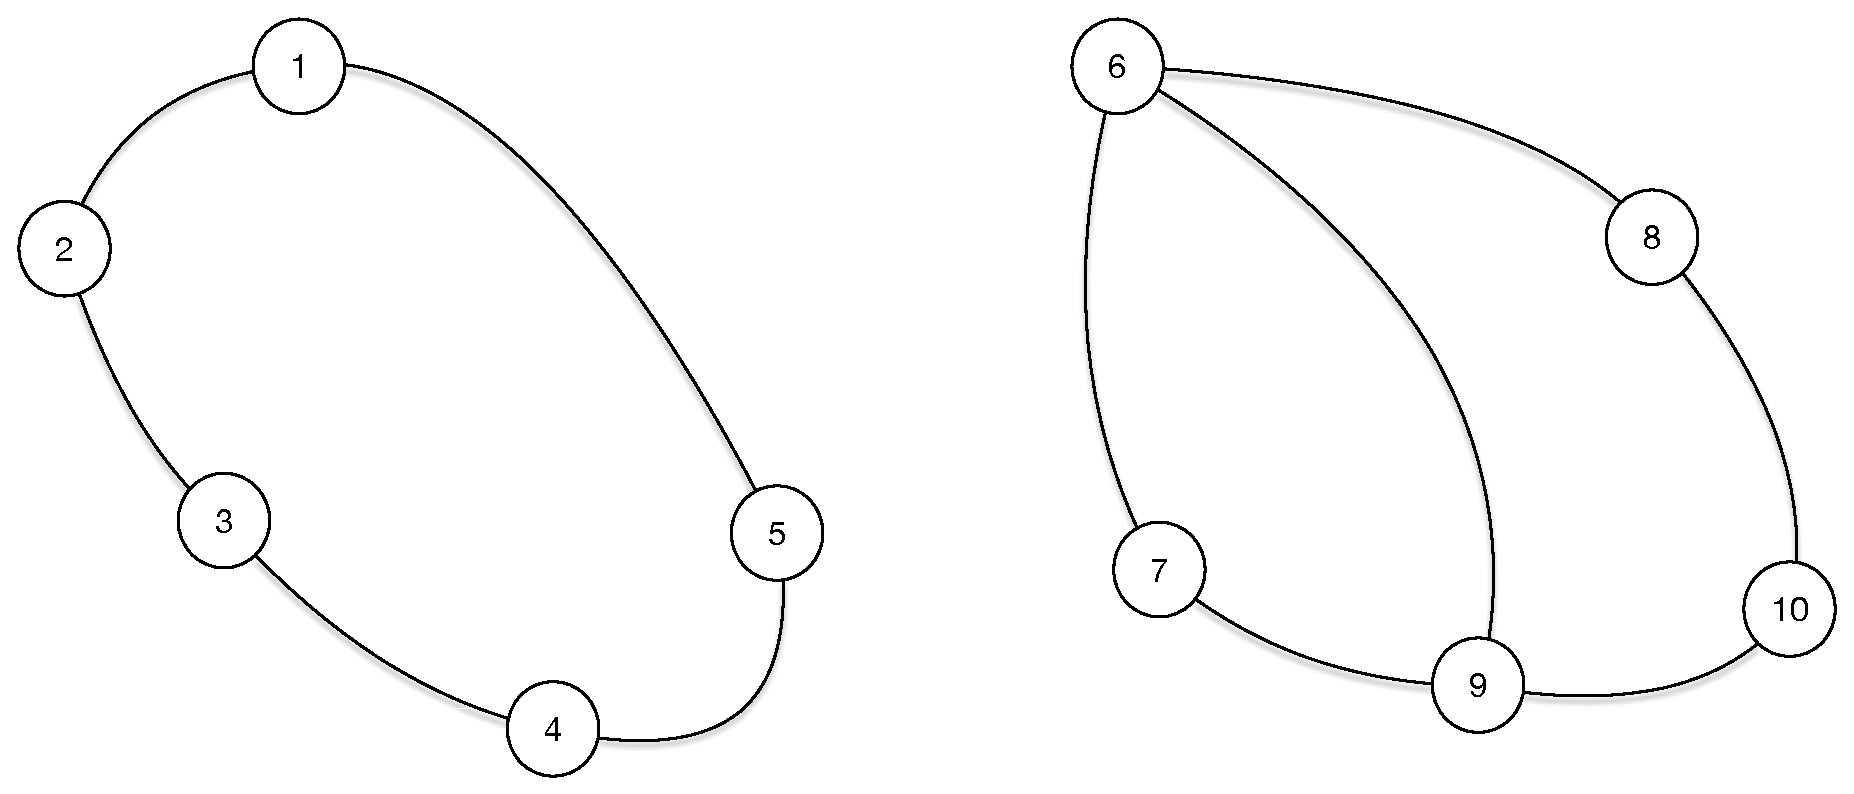
\includegraphics[width=0.7\linewidth]{images/undirected_graph_eg}
\end{figure}

\begin{lstlisting}
int main() {
  // to make sure that we can get correct graph size by graph.size()
  std::unordered_map<int, std::unordered_map<int, int>> graph = {
      {1, std::unordered_map<int, int>()}, {2, std::unordered_map<int, int>()},
      {3, std::unordered_map<int, int>()}, {4, std::unordered_map<int, int>()},
      {5, std::unordered_map<int, int>()}, {6, std::unordered_map<int, int>()},
      {7, std::unordered_map<int, int>()}, {8, std::unordered_map<int, int>()},
      {9, std::unordered_map<int, int>()}, {10, std::unordered_map<int, int>()}};

  Connect(graph, 1, 2, 1);
  Connect(graph, 2, 3, 1);
  Connect(graph, 3, 4, 1);
  Connect(graph, 4, 5, 1);
  Connect(graph, 5, 1, 1);
  Connect(graph, 6, 7, 1);
  Connect(graph, 6, 9, 1);
  Connect(graph, 7, 9, 1);
  Connect(graph, 8, 6, 1);
  Connect(graph, 8, 10, 1);
  Connect(graph, 9, 10, 1);

  std::vector<int> start_nodes = {1, 8};
  // DFS: 1 5 4 3 2 8 10 9 7 6
  std::cout << "DFS: ";
  DFS(graph, start_nodes);
  std::cout << std::endl;
  // BFS: 1 8 5 2 10 6 4 3 9 7
  std::cout << "BFS: ";
  BFS(graph, start_nodes);
  std::cout << std::endl;

  return 0;
}
\end{lstlisting}
